\chapter{Arhitektura i dizajn sustava}
		
		
		Budući da je glavna namjera sustava da funkcionira putem interneta i ima što jednostavniju uporabu od strane korisnika odlučile smo se za samostalnu jednostraničnu web aplikaciju.
		Arhitektura se može podijeliti na tri podsustava:
		\begin{itemize}
		\item Web poslužitelj
		\item Web aplikacija
		\item Baza podataka
	 	\end{itemize}
 	
 		\begin{figure}[H]
 			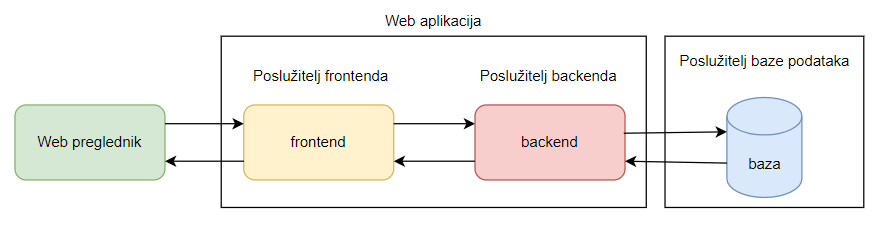
\includegraphics[scale=0.8]{slike/Arhitektura.png} %veličina slike u odnosu na originalnu datoteku i pozicija slike
 			\centering
 			\caption{Arhitektura sustava}
 			\label{fig:arhitektura}
 		\end{figure}
		
		Web preglednik je program koji korisniku omogućuje pregled web-stranica i multimedijskih sadržaja vezanih uz njih. Svaki internetski preglednik je prevoditelj. Korisnik putem web preglednika šalje zahtjev web poslužitelju.
		
		Web poslužitelj osnova je rada web aplikacije. Njegova primarna zadaća je komunikacija s aplikacijom koja se odvija preko HTTPS (engl. Hyper Text Transfer Protocol Secure) protokola, što je protokol u prijenosu informacija na webu. Poslužitelj je onaj koji pokreće web aplikaciju te joj prosljeđuje zahtjev.
		
		Korisnik koristi web aplikaciju za obrađivanje željenih zahtjeva. Web aplikacija obrađuje zahtjev te ovisno o zahtjevu, pristupa bazi podataka nakon čega preko poslužitelja vraća korisniku odgovor u web pregledniku.
		
		Programski jezik kojeg smo odabrale za izradu naše web aplikacije je Java u okviru Spring Boot te programski jezik JavaScript u React razvojnoj biblioteci. Odabrana razvojna okruženja su IntelliJ, Eclipse i  VSCode.
		Arhitektura web aplikacije je slojevita što omogućava nezavisan razvoj pojedinog dijela aplikacije, lakše ispitivanje i održavanje aplikacije te vrlo jednostavno dodavanje novih značajki u sustav. Sastoji se od pristupne i pozadinske aplikacije.
		
		Pristupna aplikacija (frontend) preko Rest API komunicira s pozadinskom aplikacijom.
		
		Pozadinska aplikacija (backend) je troslojno ustrojena:
		\begin{itemize}
		\item Repository
		\item Service
		\item Controller
		\end{itemize}
		Controller predstavlja sloj aplikacije koji obrađuje HTTP zahtjeve i priprema podatke za prikaz u JSON datoteke.
		Service je središnji sloj koji izravno upravlja podatcima, logikom i pravilima aplikacije te obavlja autentikaciju i validaciju.
		Repository šalje SQL upite bazi podataka, odnosno obavlja CRUD (Create, Retrieve, Update and Delete) operacije.
		

				
		\section{Baza podataka}
			
			
			
		Za potrebe našeg sustava koristit ćemo relacijsku bazu podataka čija je gradivna jedinka relacija, odnosno dvodimenzionalna imenovana tablica sa skupom atributa - imenovanim stupcima tablice. Relacijska baza podataka omogućava jednostavno pohranjivanje i upravljanje podatcima. Baza podataka ove aplikacije sastoji se od sljedećih entiteta:
		
		\begin{itemize}
		    \item   UserAccount
		    \item   Conference
		    \item   Multimedia
		    \item   SpecialEvent
		    \item   DataGroup
		    \item   conferenceDataGroup
		    \item   operationalAdmins
		    \item   pending
		    \item   attendees
                \item   users
		\end{itemize}

		
			\subsection{Opis tablica}
			
			\textbf{UserAccount} Ovaj entitet opisuje korisnika konferencije i njegov račun s kojim se prijavljuje u aplikaciju. Sadrži atribute idUserAccount, address, companyName, country, detailsOfParticipation, email, enabled, firstAndLastName, isMainAdmin, isOperativeAdmin, isParticipant, isSystemOwner, phoneNumber, username, password i idConference. Postoje četiri vrste korisnika, vlasnik sustava, glavni admin, operativni admin te sudionik konferencije.
			
		
				
				\begin{longtblr}[
					label=none,
					entry=none
					]{
						width = \textwidth,
						colspec={|X[13,l]|X[9, l]|X[20, l]|}, 
						rowhead = 1,
					} %definicija širine tablice, širine stupaca, poravnanje i broja redaka naslova tablice
					\hline \multicolumn{3}{|c|}{\textbf{UserAccount}}	 \\ \hline[3pt]
					\SetCell{LightGreen}idUserAccount & INT	&  	jedinstveni identifikator korisnika  	\\ \hline
					address	& VARCHAR &  adresa 	\\ \hline 
					companyName & VARCHAR &   ime tvrtke\\ \hline 
					country & VARCHAR	&  		država\\ \hline
					detailsOfParticipation & VARCHAR	&  	uloga	\\ \hline
					email & VARCHAR	&  	email	\\ \hline
                        enabled & BOOLEAN	&  	potvrđen račun	\\ \hline
					firstAndLastName & VARCHAR	&  	ime i prezime	\\ \hline
					isMainAdmin & BOOLEAN	&  	je li glavni admin\\ \hline
					isOperativeAdmin & BOOLEAN	&  je li operativni admin		\\ \hline
					isParticipant & BOOLEAN	& je li participant  		\\ \hline
					isSystemOwner & BOOLEAN	&  je li vlasnik sustava		\\ \hline
					phoneNumber & VARCHAR	&  broj mobitela		\\ \hline
					username & VARCHAR	&  	korisničko ime	\\ \hline
					password & VARCHAR	&  	lozinka	\\ \hline
				\end{longtblr}

                \vspace{8mm}
				
				
				\textbf{Conference} Ovaj entitet opisuje konferenciju. Sadrži atribute idConference, city, country, dateStart, dateEnd, description, topics, name,
				mainAdminIdUserAccount i systemOwnerIdUserAccount. Ovaj entitet je u dvije veze \textit{One-to-Many} sa entitetom UserAccount preko atributa idConference, jedna veza predstavlja operativne admine, a druga participante konferencije, također je u vezi \textit{One-to-Many} sa entitetom dataGroup preko atributa idConference, \textit{One-to-Many} sa entitetom SpecialEvent preko atributa idConference te je u vezi \textit{One-to-Many} sa entitetom Multimedia preko atributa idConference.
			
				
				\begin{longtblr}[
					label=none,
					entry=none
					]{
						width = \textwidth,
						colspec={|X[17,l]|X[7, l]|X[20, l]|}, 
						rowhead = 1,
					} %definicija širine tablice, širine stupaca, poravnanje i broja redaka naslova tablice
					\hline \multicolumn{3}{|c|}{\textbf{Conference}}	 \\ \hline[3pt]
					\SetCell{LightGreen}idConference & INT	&  	jedinstveni identifikator konferencije  	\\ \hline
					city	& VARCHAR & grad u kojem se održava  	\\ \hline 
                        country	& VARCHAR & država u kojoj se održava  	\\ \hline 
                        dateStart	& DATE & datum početka konferencije 	\\ \hline
					dateEnd & DATE &  datum završetka konferencije \\ \hline 
					description	& VARCHAR &  kratak opis konferencije 	\\ \hline
                        topics	& VARCHAR &  teme 	\\ \hline 
					name & VARCHAR &   naziv grupe podaataka\\ \hline 
					\SetCell{LightBlue}mainAdminIdUserAccount & INT &  id glavnog admina sustava \\ \hline 
					\SetCell{LightBlue}systemOwnerIdUserAccount & INT &  id vlasnika sustava \\ \hline 
				\end{longtblr}

                \vspace{8mm}
				
				
				\textbf{Multimedia} Ovaj entitet opisuje multimedijske sadržaje snimane od strane ovlaštenog fotografa za određenu konferenciju. Sadrži atribute idMultimedia, url, date i idConference.  Ovaj entitet je u vezi \textit{Many-to-One} sa entitetom Conference preko atributa idConference.
				
				\begin{longtblr}[
					label=none,
					entry=none
					]{
						width = \textwidth,
						colspec={|X[7,l]|X[6, l]|X[20, l]|}, 
						rowhead = 1,
					} %definicija širine tablice, širine stupaca, poravnanje i broja redaka naslova tablice
					\hline \multicolumn{3}{|c|}{\textbf{Multimedia}}	 \\ \hline[3pt]
					\SetCell{LightGreen}idMultimedia & INT	&  	jedinstveni identifikator multimedijskog sadržaja  	\\ \hline
					url	& VARCHAR &  link na drive gdje je pohranjena multimedia	\\ \hline 
					date	& DATETIME &   datum nastanka	\\ \hline 
					\SetCell{LightBlue}idConference	& INT &   id konferencije kojoj pripada	\\ \hline 
				\end{longtblr}

                \vspace{8mm}
				
				
				
				\textbf{SpecialEvent} Ovaj entitet opisuje posebna događanja tijekom neke konferencije. Sadrži atribute idSpecialEvent, capacity, type, message i idConference.  Ovaj entitet je u vezi \textit{Many-to-One} sa entitetom Conference preko atributa idSpecialEvent te je u dvije veze \textit{Many-to-Many} sa entitetom UserAccount preko atributa idSpecialEvent. Jedna veza opisuje korisnike koji su prijavljeni za sudjelovanje na posebnom događaju, a druga opisuje korisnike koji su na čekanju za sudjelovanje zbog popunjenih kapaciteta.
			
				
				\begin{longtblr}[
					label=none,
					entry=none
					]{
						width = \textwidth,
						colspec={|X[7,l]|X[6, l]|X[20, l]|}, 
						rowhead = 1,
					} %definicija širine tablice, širine stupaca, poravnanje i broja redaka naslova tablice
					\hline \multicolumn{3}{|c|}{\textbf{SpecialEvent}}	 \\ \hline[3pt]
					\SetCell{LightGreen}idSpecialEvent & INT	&  	jedinstveni identifikator posebnog događaja 	\\ \hline
					capacity	& INT &   maksimalan broj sudionika	\\ \hline 
					type & VARCHAR &  tip događaja \\ \hline 
					message & VARCHAR &  kratka poruka o događaju \\ \hline 
                        \SetCell{LightBlue}idConference	& INT &   id konferencije kojoj pripada	\\ \hline 
				\end{longtblr}

                \vspace{8mm}
				
				
				\textbf{DataGroup} Ovaj entitet opisuje grupu podataka o nekoj konferenciji (raspored, zbornik radova i sl.). Sadrži atribute idDataGroup, groupName, data i idConference.  Ovaj entitet je u vezi \textit{Many-to-One} sa entitetom Conference preko atributa idDataGroup.
				
				\begin{longtblr}[
					label=none,
					entry=none
					]{
						width = \textwidth,
						colspec={|X[10,l]|X[6, l]|X[20, l]|}, 
						rowhead = 1,
					} %definicija širine tablice, širine stupaca, poravnanje i broja redaka naslova tablice
					\hline \multicolumn{3}{|c|}{\textbf{DataGroup}}	 \\ \hline[3pt]
					\SetCell{LightGreen}idDataGroup & INT	&  	jedinstveni identifikator grupe podataka  	\\ \hline
					data	& VARCHAR &   	podatak za određenu grupu podataka (može biti tekst ili datoteka)\\ \hline 
					groupName	& VARCHAR &   	naziv\\ \hline
				\end{longtblr}

                \vspace{8mm}
				
				
				
				\textbf{ConferenceDataGroup} Ovaj entitet opisuje odnos između entiteta Conference i DataGroup. Sadrži atribute idDataGroup i idConference.  Ovaj entitet je u vezi \textit{Many-to-One} sa entitetom Conference preko atributa idConference te u vezi \textit{Many-to-One} sa entitetom DataGroup preko atributa idDataGroup.
				
				\begin{longtblr}[
					label=none,
					entry=none
					]{
						width = \textwidth,
						colspec={|X[13,l]|X[6, l]|X[20, l]|}, 
						rowhead = 1,
					} %definicija širine tablice, širine stupaca, poravnanje i broja redaka naslova tablice
					\hline \multicolumn{3}{|c|}{\textbf{ConferenceDataGroup}}	 \\ \hline[3pt]
					\SetCell{LightGreen}idDataGroup & INT	&  	jedinstveni identifikator grupe podataka  	\\ \hline
					\SetCell{LightGreen}idConference	& INT &   jedinstveni identifikator konferencije   	\\ \hline
				\end{longtblr}

                \vspace{8mm}
				
				\textbf{OperationalAdmins} Ovaj entitet opisuje odnos između entiteta Conference i UserAccount, a predstavlja operativne admine. Sadrži atribute idUserAccount i idConference.  Ovaj entitet je u vezi \textit{Many-to-One} sa entitetom Conference preko atributa idConference te u vezi \textit{Many-to-One} sa entitetom UserAccount preko atributa idUserAccount.
				
				\begin{longtblr}[
					label=none,
					entry=none
					]{
						width = \textwidth,
						colspec={|X[17,l]|X[6, l]|X[20, l]|}, 
						rowhead = 1,
					} %definicija širine tablice, širine stupaca, poravnanje i broja redaka naslova tablice
					\hline \multicolumn{3}{|c|}{\textbf{OperationalAdmins}}	 \\ \hline[3pt]
					\SetCell{LightGreen}idUserAccount & INT	&  	jedinstveni identifikator operativnog admina  	\\ \hline
					\SetCell{LightGreen}idConference	& INT &   jedinstveni identifikator konferencije   	\\ \hline
				\end{longtblr}

                \vspace{8mm}
				
				
				\textbf{Users} Ovaj entitet opisuje odnos između entiteta Conference i UserAccount, a predstavlja participante konferencije. Sadrži atribute idUserAccount i idConference.  Ovaj entitet je u vezi \textit{Many-to-One} sa entitetom Conference preko atributa idConference te u vezi \textit{Many-to-One} sa entitetom UserAccount preko atributa idUserAccount.
				
				\begin{longtblr}[
					label=none,
					entry=none
					]{
						width = \textwidth,
						colspec={|X[17,l]|X[6, l]|X[20, l]|}, 
						rowhead = 1,
					} %definicija širine tablice, širine stupaca, poravnanje i broja redaka naslova tablice
					\hline \multicolumn{3}{|c|}{\textbf{Users}}	 \\ \hline[3pt]
					\SetCell{LightGreen}idUserAccount & INT	&  	jedinstveni identifikator participanta konferencije  	\\ \hline
					\SetCell{LightGreen}icConference	& INT &   jedinstveni identifikator konferencije   	\\ \hline
				\end{longtblr}

                \vspace{8mm}

                
				\textbf{VerificationToken} Ovaj entitet opisuje tokene koji se koriste pri potvrdi računa mailom. Ovaj entitet je u vezi \textit{Many-to-One} sa entitetom UserAccount preko atributa idUserAccount.
				
				\begin{longtblr}[
					label=none,
					entry=none
					]{
						width = \textwidth,
						colspec={|X[17,l]|X[8, l]|X[20, l]|}, 
						rowhead = 1,
					} %definicija širine tablice, širine stupaca, poravnanje i broja redaka naslova tablice
					\hline \multicolumn{3}{|c|}{\textbf{VerificationToken}}	 \\ \hline[3pt]
					\SetCell{LightGreen}idToken & INT	&  	jedinstveni identifikator tokena  	\\ \hline
					createdDate	& DATE &   datum i vrijeme nastanka tokena   	\\ \hline
                        expiryDate	& DATE &   datum i vrijeme prestanka valjanosti tokena   	\\ \hline
                        token	& VARCHAR &   token   	\\ \hline
                        \SetCell{LightBlue}idUserAccount	& INT &   id korisničkog računa za kojeg je token generiran   	\\ \hline
				\end{longtblr}

                \vspace{8mm}

                
            


                \textbf{SpecialEventAttendees} Ovaj entitet opisuje odnos između entiteta SpecialEvent i UserAccount, a predstavlja participante koji su prijavljeni na neki specijalni događaj. Sadrži atribute idUserAccount i idSpecialEvent.  Ovaj entitet je u vezi \textit{Many-to-One} sa entitetom SpecialEvent preko atributa idSpecialEvent te u vezi \textit{Many-to-One} sa entitetom UserAccount preko atributa idUserAccount.
				
				\begin{longtblr}[
					label=none,
					entry=none
					]{
						width = \textwidth,
						colspec={|X[17,l]|X[6, l]|X[20, l]|}, 
						rowhead = 1,
					} %definicija širine tablice, širine stupaca, poravnanje i broja redaka naslova tablice
					\hline \multicolumn{3}{|c|}{\textbf{SpecialEventAttendees}}	 \\ \hline[3pt]
					\SetCell{LightGreen}idUserAccount & INT	&  	jedinstveni identifikator participanta konferencije  	\\ \hline
					\SetCell{LightGreen}idSpecialEvent	& INT &   jedinstveni identifikator specijalnog događaja   	\\ \hline
				\end{longtblr}

                \vspace{8mm}


                \textbf{SpecialEventPending} Ovaj entitet opisuje odnos između entiteta SpecialEvent i UserAccount, a predstavlja participante koji su se htjeli prijaviti na specijalni događaj, ali su stavljeni na čekanje zbog popunjenih kapaciteta na tom događaju. Sadrži atribute idUserAccount i idSpecialEvent.  Ovaj entitet je u vezi \textit{Many-to-One} sa entitetom SpecialEvent preko atributa idSpecialEvent te u vezi \textit{Many-to-One} sa entitetom UserAccount preko atributa idUserAccount.
				
				\begin{longtblr}[
					label=none,
					entry=none
					]{
						width = \textwidth,
						colspec={|X[17,l]|X[6, l]|X[20, l]|}, 
						rowhead = 1,
					} %definicija širine tablice, širine stupaca, poravnanje i broja redaka naslova tablice
					\hline \multicolumn{3}{|c|}{\textbf{SpecialEventPending}}	 \\ \hline[3pt]
					\SetCell{LightGreen}idUserAccount & INT	&  	jedinstveni identifikator participanta konferencije  	\\ \hline
					\SetCell{LightGreen}idSpecialEvent	& INT &   jedinstveni identifikator specijalnog događaja   	\\ \hline
				\end{longtblr}

                \vspace{8mm}
				
				
				
				
			\subsection{Dijagram baze podataka}
				\begin{figure}[H]
			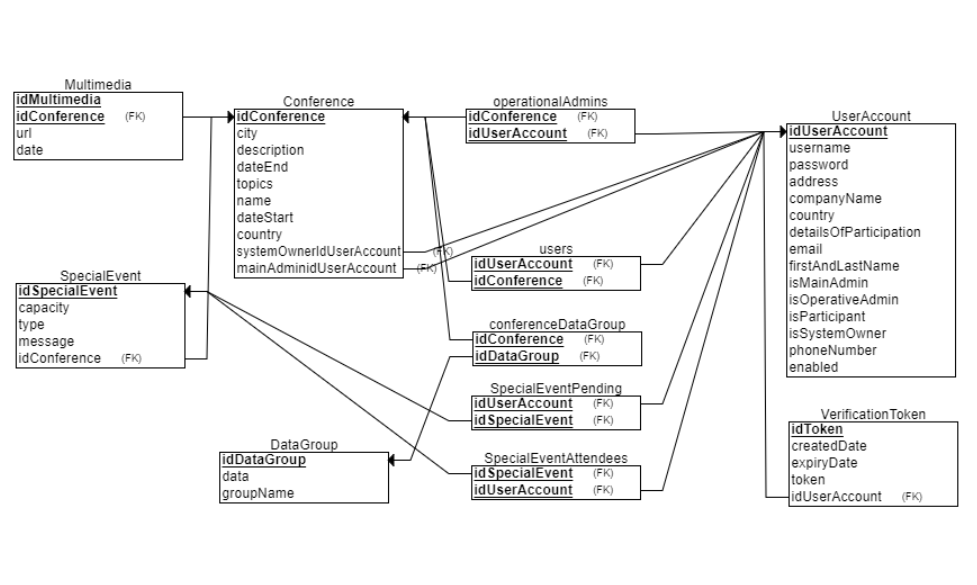
\includegraphics[scale=0.85]{slike/RelModel.PNG} %veličina slike u odnosu na originalnu datoteku i pozicija slike
			\centering
			\caption{Relacijski model baze}
			\label{fig:promjene}
		\end{figure}
			
			\eject
			
			
		
			\section{Dijagram razreda}

			\text Na slikama 4.3, 4.4, 4.5 i 4.6 su prikazani razredi koji pripadaju backend dijelu arhitekture. Slika 4.3 prikazuje razred DTO \textit{(Data Transfer Object)} razrede.
			Na slici 4.4. prikazan je dijagram Modela, oni predstavljaju entitete naše baze podataka, na tom dijagramu također možemo vidjeti i međusobnu ovisnost entiteta. Zatim slike 4.5 i 4.6 prikazuju Kontrolere i Service, metode u Kontrolerima manipuliraju s DTO podatcima, primaju zahtjeve s frontend-a koje dalje šalje na Service gdje se zahtjev obrađuje. Povratna informacija koja se generira u Service se ponovno vraća preko Kontrolera koji vraća JSON datoteku na frontend. 
			

			\begin{figure}[H]
			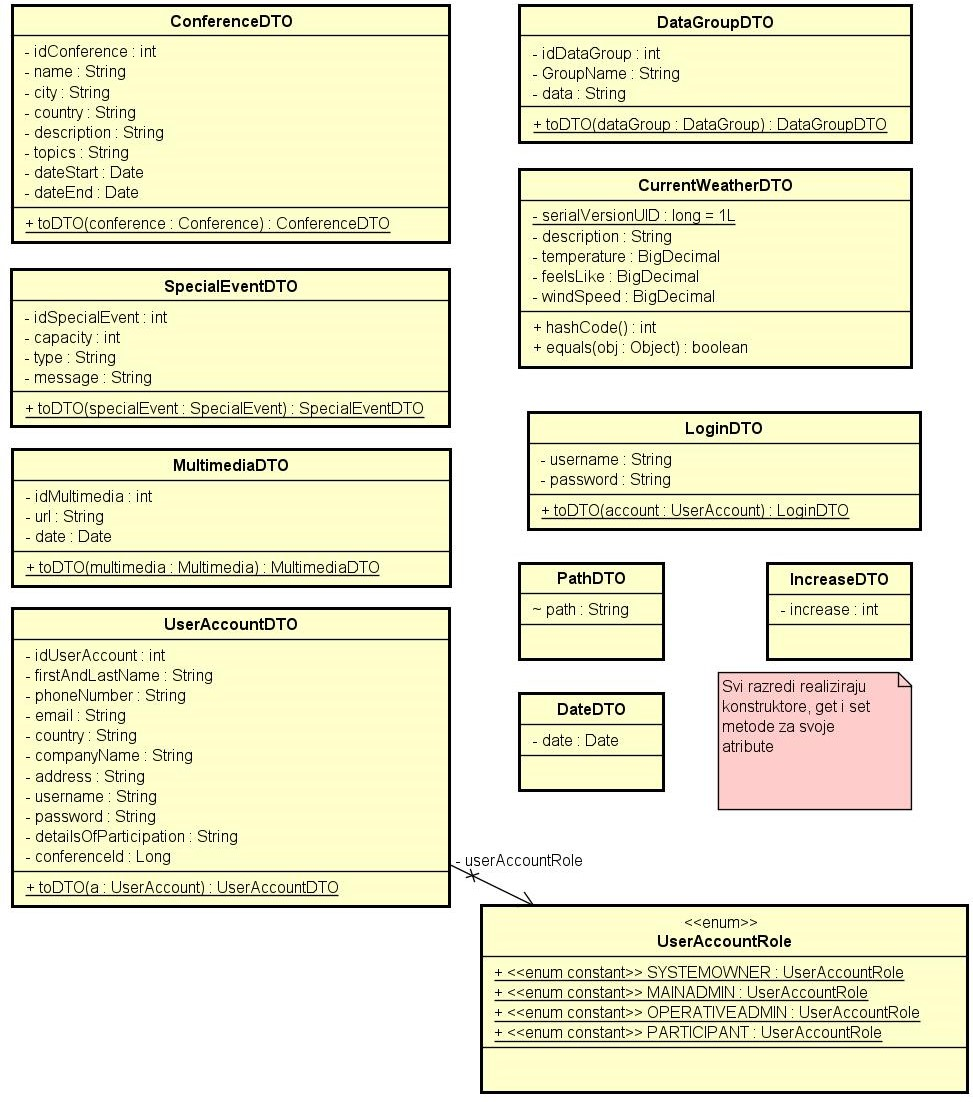
\includegraphics[width=\textwidth]{slike/DTO Dijagram.jpg}
			\centering
			\caption{Dijagram razreda - DTO}
			\label{fig:}
			\end{figure}
			
			\newpage

			\begin{figure}[H]
			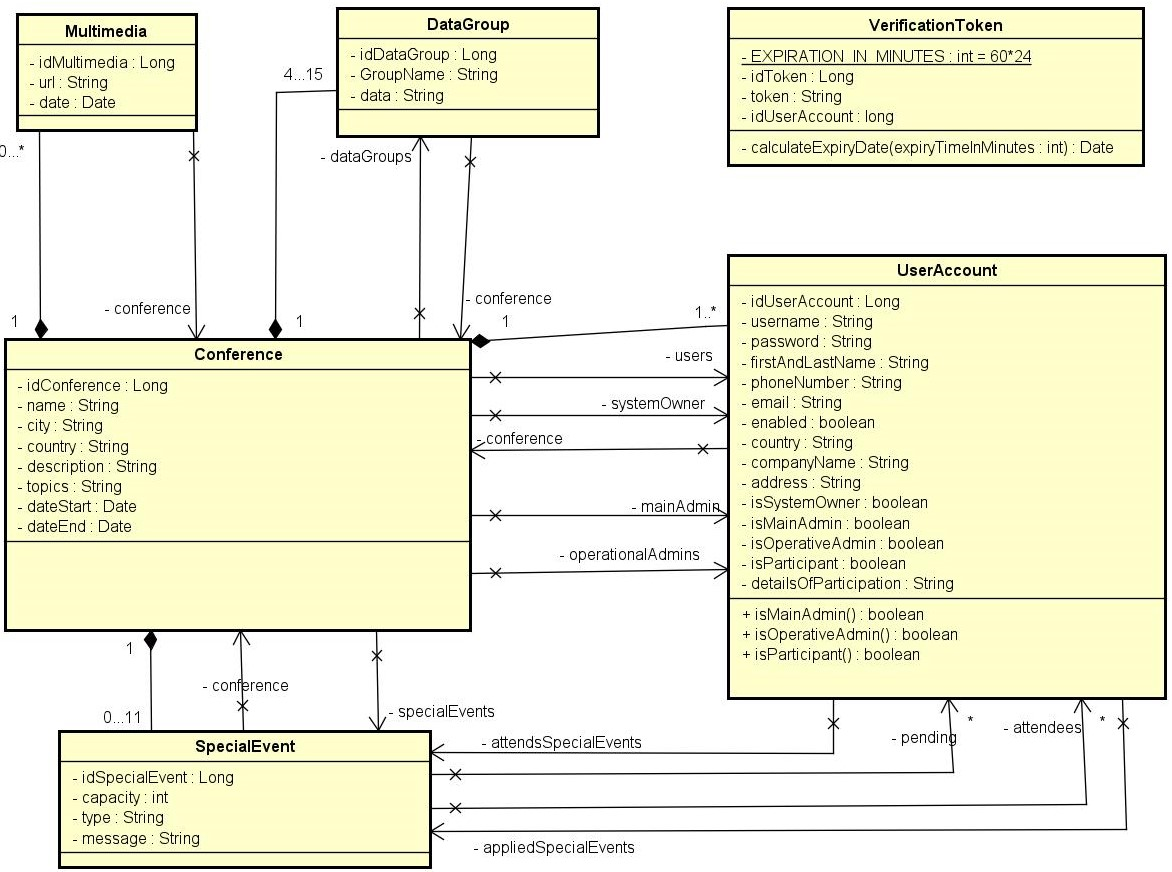
\includegraphics[width=\textwidth]{slike/Model diagram.jpg}
			\centering
			\caption{Dijagram razreda - Modeli}
			\label{fig:dijagram_razreda_modeli}
			\end{figure}
			
			\newpage


			\begin{figure}[H]
			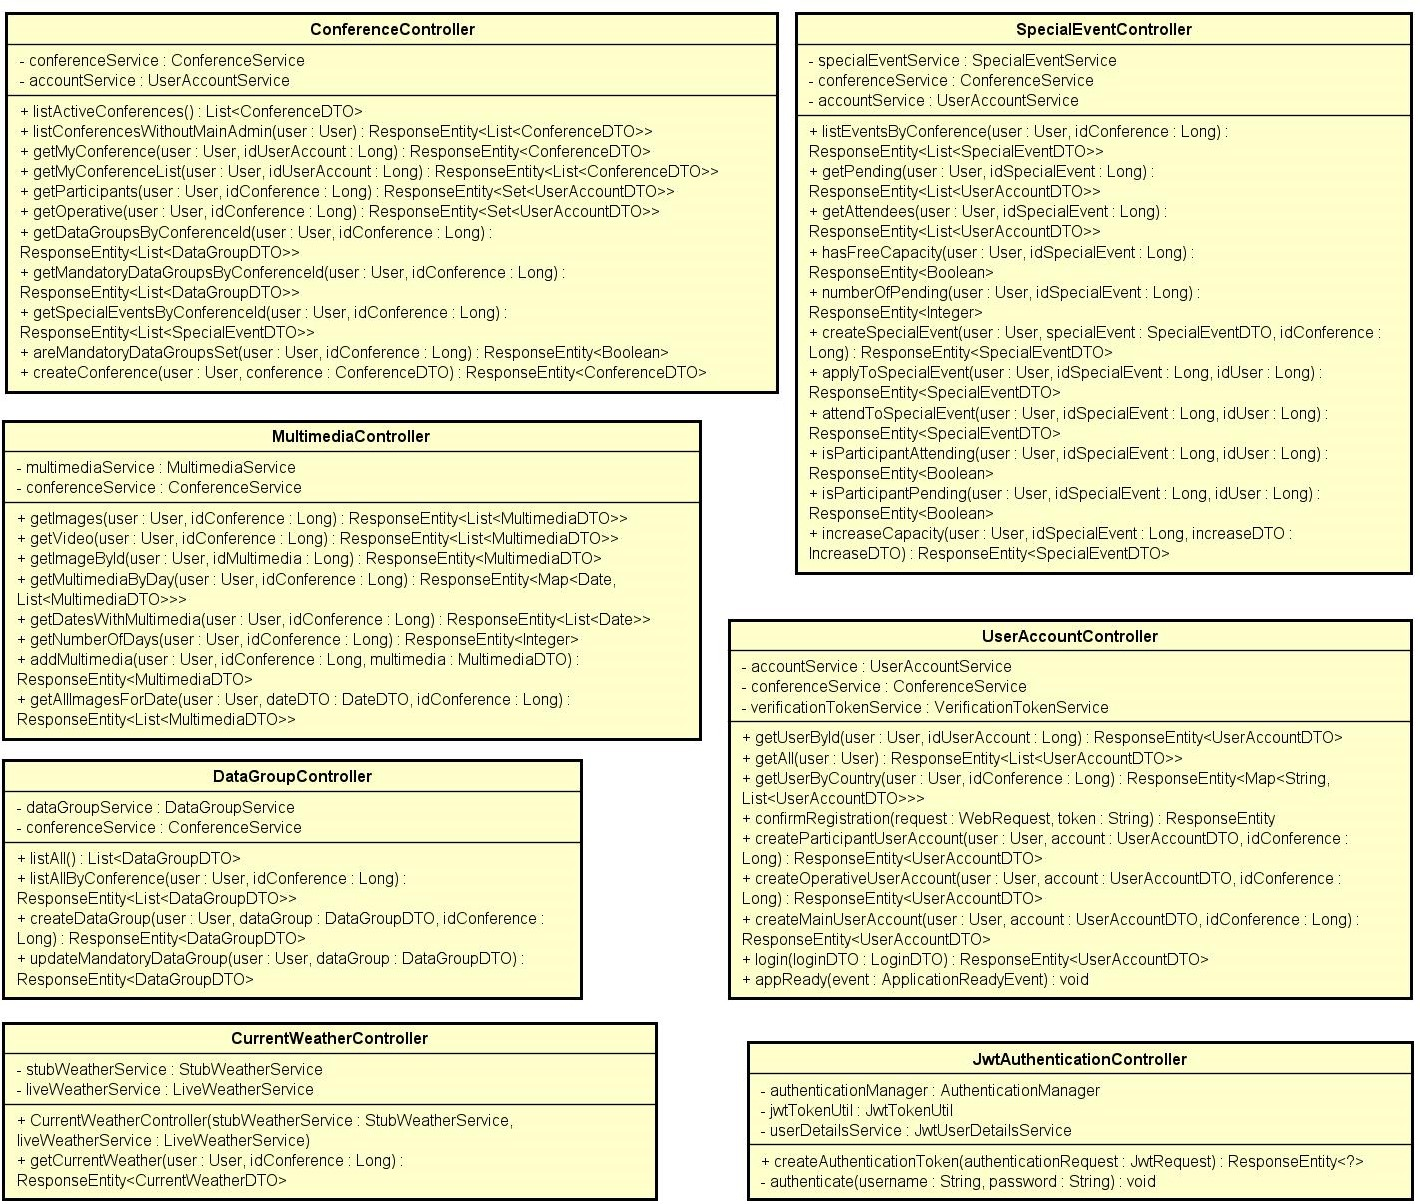
\includegraphics[width=\textwidth]{slike/Controller Dijagram.jpg}
			\centering
			\caption{Dijagram razreda - Kontroleri}
			\label{fig:dijagram_razreda_kontroleri}
			\end{figure}
			
			\newpage

			 \begin{figure}[H]
			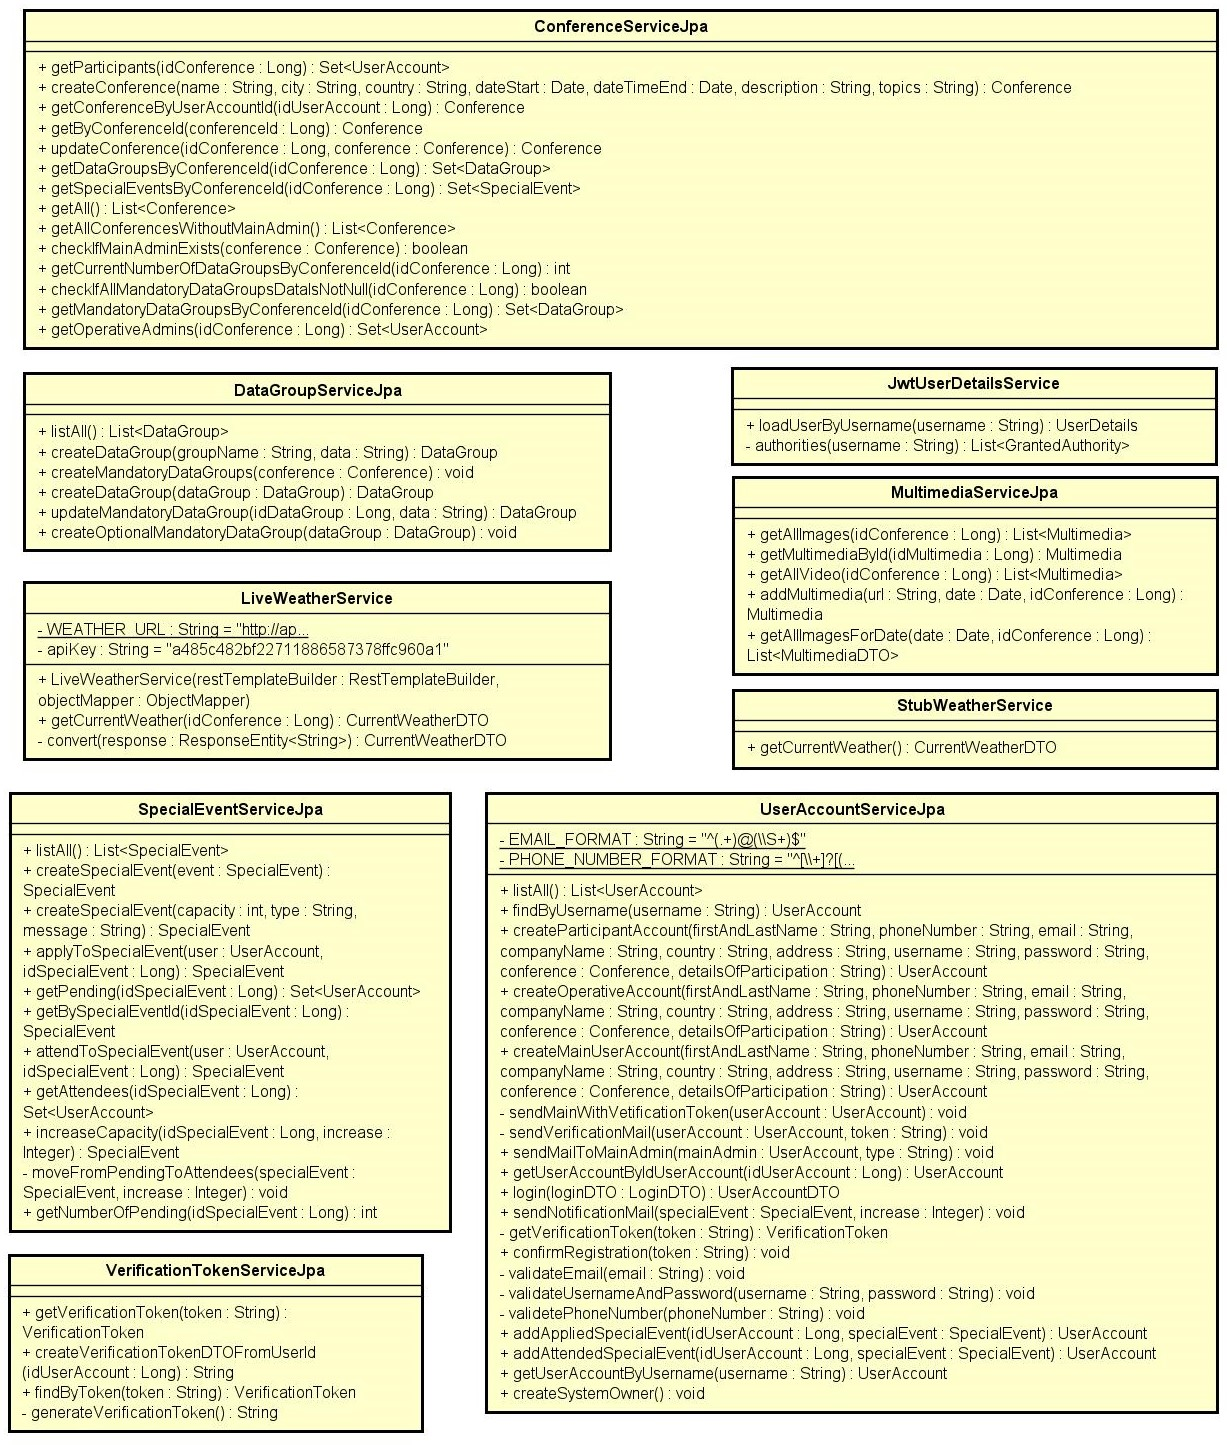
\includegraphics[width=\textwidth]{slike/ServiceImpl Dijagram.jpg}
			\centering
			\caption{Dijagram razreda -  Service}
			\label{fig:dijagram_razreda_service}
			\end{figure}
			
			\newpage
			
	
			\eject
		
		\section{Dijagram stanja}
			
			
Dijagram stanja prikazuje stanja objekta te prijelaze iz jednog stanja u drugo temeljene na dogadajima. Na slici 4.7 prikazan je dijagram stanja za registriranog main admina. Nakon prijave prvo se prikazuje početni izbornik koji nudi tri opcije : \textit{Home, My Conference} i \textit{Create Operative Admin}. Klikom na "Home" poziva se početna stranica na kojoj se prikazuju aktivne konferencije. Klikom na "Create Operative Admin" prikaže se forma za kreiranje operativnog admina. Klikom na \"My Conference" prikažu se podatci o konferenciji. Main admin tu ima mogućnosti stvoriti novu grupu podataka klikom na "New Data Group". Ima mogućnsot pregleda svih sudionika i operativnih admina klikom na \textit{Show Attendees}. Klikom na "Special Events" main admin dobiva prikaz svih događaja za tu konferenciju gdje može odabrati stvaranje novog događaja klikom na "New Special Event". Također može povećati kapacitet za određeni događaj. Ako je lista čekanja prazna, povećanje kapaciteta će biti odbijeno, ako lista čekanja nije prazna kapacitet će se povećati. Iz stanja \textit{Prikaz Moje Konferencije} može pristupiti i multimediji klikom na "See Multimedia", dobiva prikaz direktorija raspoređeni po danima, klikom na direktorij prikažu se slike tog dana.

                \begin{figure}[H]
			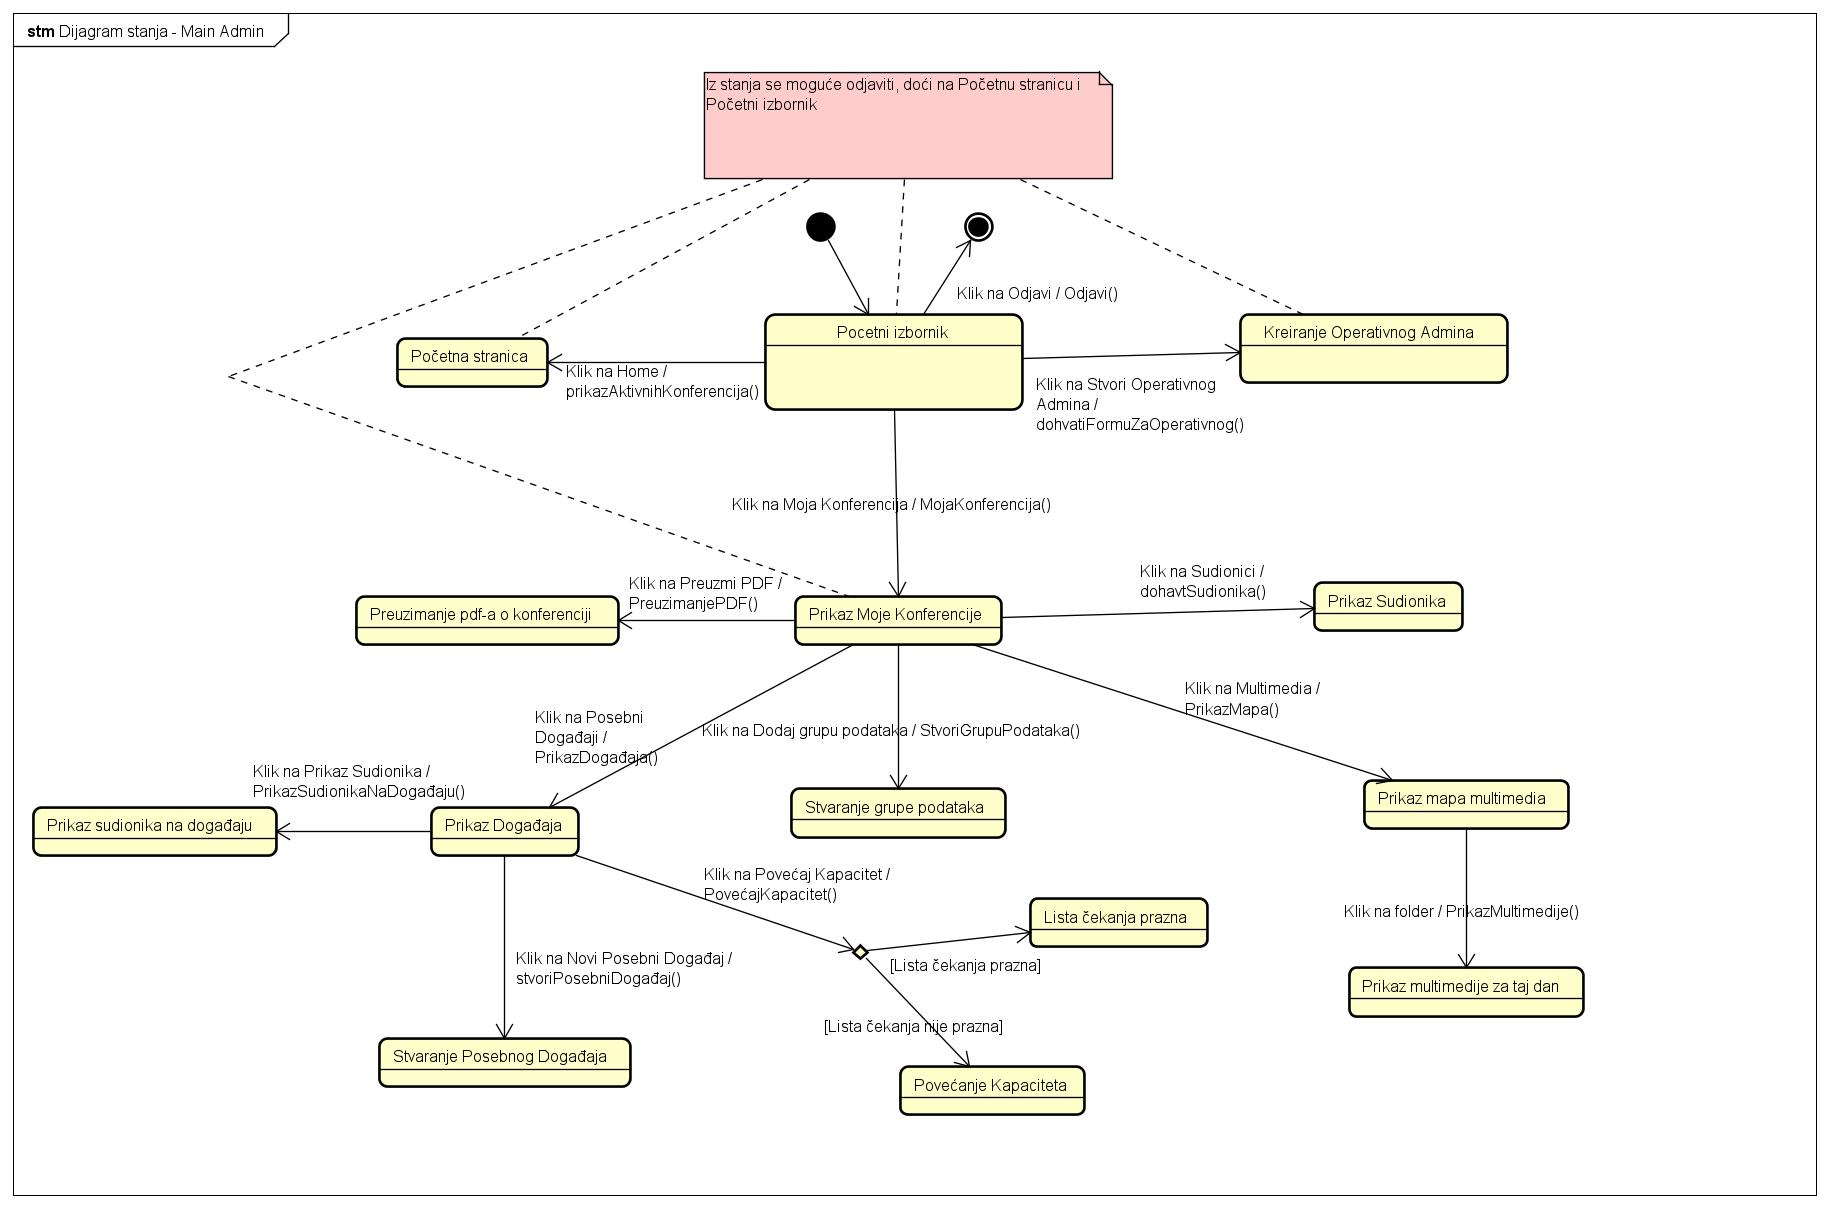
\includegraphics[width = \textwidth]{slike/Dijagram stanja - Main Admin.jpg}
			\centering
			\caption{Dijagram stanja - Main Admin}
			\label{fig:dijagram-stanja-main-admin}
			\end{figure}
			
			
			\eject 
		
			\section{Dijagram aktivnosti}
			
			\textbf{Vlasnik sustava - kreiranje konferencije i glavnog admina}\\

		   \text Na dijagramu aktivnosti prikazan je proces stvaranja konferencije i main admina. Vlasnik sustava prijavljuje se u sustav, odabire gumb za kreiranje konferencije, te unosi podatke o konferenciji. Nakon toga otvara se obrazac za unos podataka o main adminu.


		   \begin{figure}[H]
		   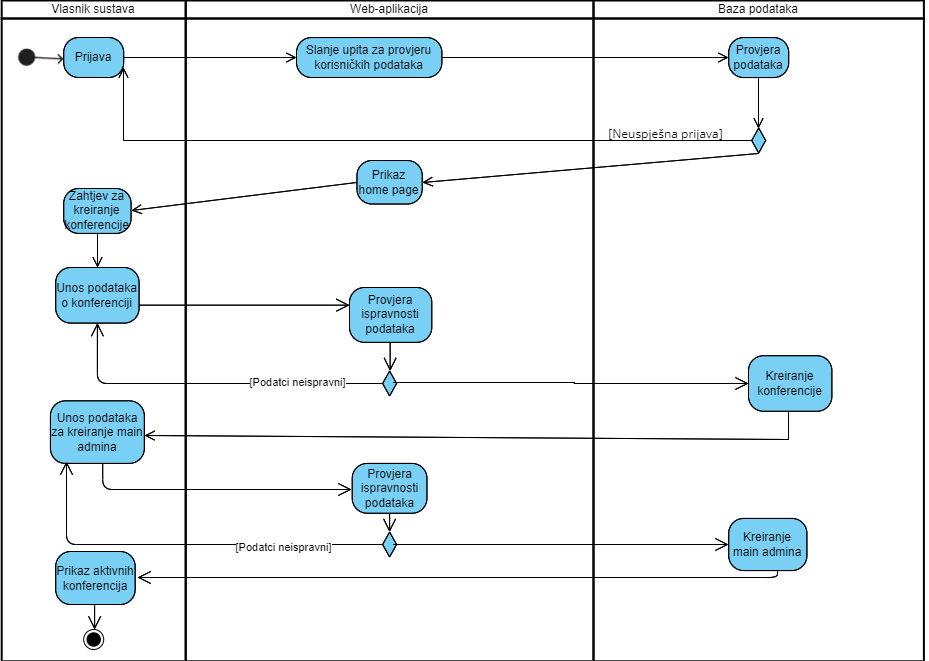
\includegraphics[scale=0.65]{slike/Dijagram aktivnosti - system owner.png} %veličina
		   
		   \centering
		   \caption{Kreiranje konferencije i glavnog admina}
		   \label{fig:dijagram_aktivnosti_vlasnik_sustava}
		   \end{figure}

  \textbf{Glavni admin - unos grupa podataka}\\

		   \text Na dijagramu aktivnosti prikazan je proces unosa grupa podataka. Glavni admin prijavljuje se u sustav, odabire gumb "My conference", te unosi obavezne grupe podataka. Nakon toga može stvarati i opcionalne grupe po dataka. 


		   \begin{figure}[H]
		   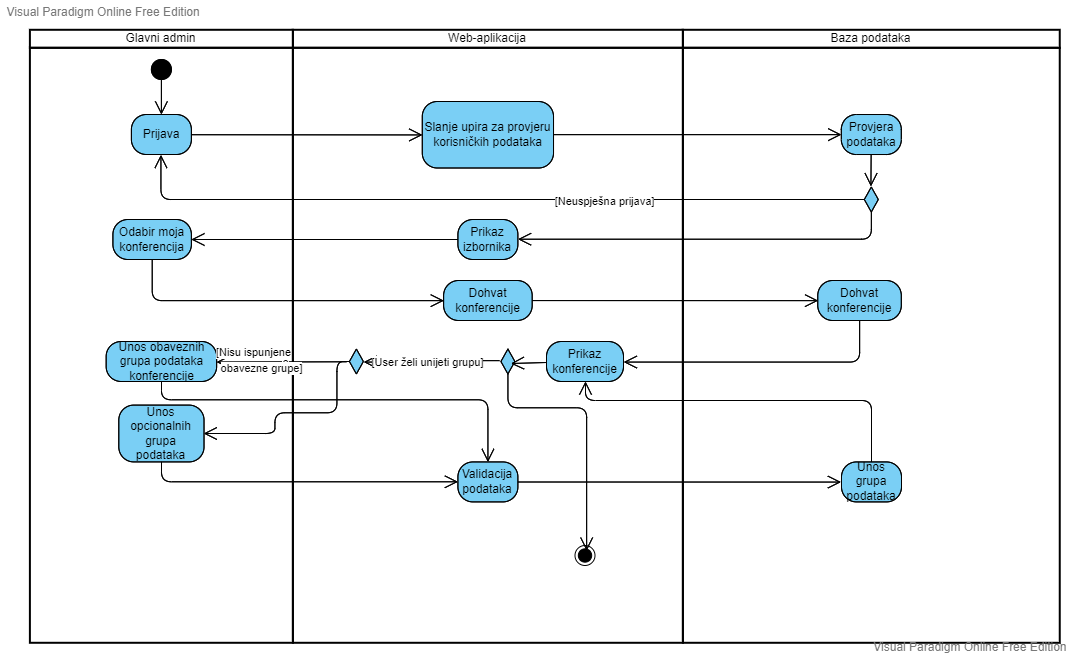
\includegraphics[scale=0.45]{slike/Main admin - unos grupa podataka.png} %veličina
		   
		   \centering
		   \caption{Unos grupa podataka}
		   \label{fig:dijagram_aktivnosti_glavni_admin}
		   \end{figure}

   \textbf{Operativni admin - kreiranje korisnika}\\

		   \text Na dijagramu aktivnosti prikazan je proces kreiranja korisnika. Operativni admin prijavljuje se u sustav, odabire gumb "Create user", te mu se otvara obrazac za popunjavanje podataka o korisniku. Nakon uspješnog unosa korisnika, korisnik mora potvrditi svoj korisnički račun mailom.  


		   \begin{figure}[H]
		   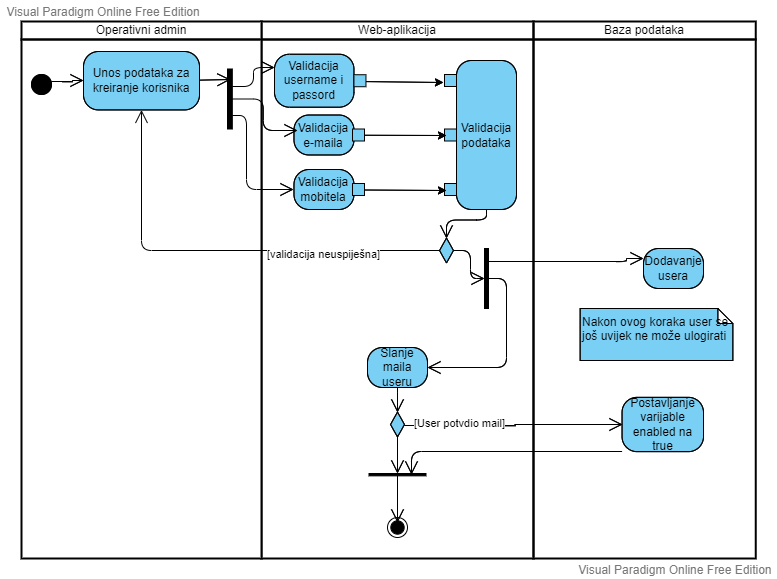
\includegraphics[scale=0.60]{slike/Creating user.vpd.png} %veličina
		   
		   \centering
		   \caption{Kreiranje korisnika}
		   \label{fig:dijagram_aktivnosti_operativni_admin}
		   \end{figure}

  \textbf{Korisnik - prijava na specijalni event}\\

		   \text Na dijagramu aktivnosti prikazan je proces prijave korisnika na specijalni event. Kada korisnik odabere gumb "Special event", otvara mu se lista specijalnih eventova na koje se može prijaviti. Ako na na specijalnom eventu ima mjesta, korisnik se automatski dodaje na listu prijavljenih korisnika za specijalni event. U slučaju da su sva mjesta na specijalnom eventu popunjena, korisnika se o tome obavještava. U slučaju da se naknadno poveća broj slobodnih mjesta na specijalnom eventu, korisnika se mailom obavještava da je sada na listi prijavljenih korisnika.  


		   \begin{figure}[H]
		   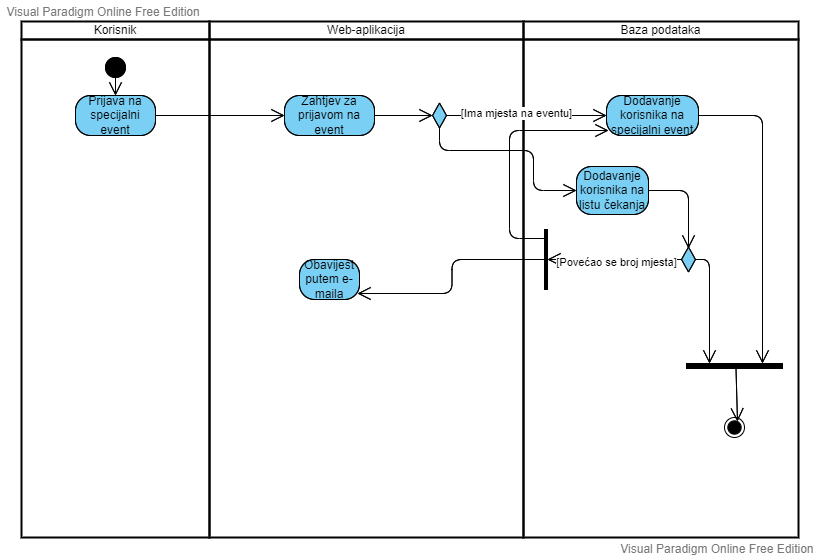
\includegraphics[scale=0.55]{slike/Prijava na special event.vpd.png} %veličina
		   
		   \centering
		   \caption{Prijava na specijalni event}
		   \label{fig:dijagram_aktivnosti_korisnik}
		   \end{figure}
		   
		   
		   \eject

		\section{Dijagram komponenti}

     \textbf{Dijagram komponenti}\\
				
				{Prikazani dijagram komponenti prikazuje organizaciju i međuovisnost komponenti i odnose prema okolini. Sustavu se pristupa preko dva različita sučelja. Preko sučelja za dohvat HTML, CSS i JS datoteka poslužuju se datoteke koje pripadaju frontend dijelu aplikacije. To je sučelje zahtjevano sučelje za React View komponentu budući da preko njega ostvaruje prikaz i osvježavanje frontenda. Router je komponenta koja na upit s url-om određuje koja datoteka će se poslužiti na sučelje. Svaka datoteka predstavlja jednu stranicu aplikacije, tj. JavaScript kod te datoteke. Sve JavaScript datoteke ovise o React biblioteci iz koje dohvaćaju gotove komponente kao što su gumbi, forme i slično. Preko sučelja za dohvat JSON podataka pristupa se REST API komponenti. REST API poslužuje podatke koji pripadaju backend dijelu aplikacije. JPA(Java persistance API) je zadužen za dohvaćanje tablica iz baze podataka pomoću SQL upita. Sučelje za komunikaciju s JPA koristi Repository razred Swing aplikacije kako bi na zahtjev iz Service komponente mogla poslati upit bazi podataka. Podatci koji su pristigli iz baze se šalju dalje arhitekturi u obliku DTO (Data transfer object) iz Service prema Contolleru i dalje prema frontend dijelu aplikacije. Reactview komponenta preko dostupnih sučelja komunicira sa Kokeferencije aplikacijom te ovisno o korisnikovim akcijama osvježava prikaz i dohvaća nove podatke ili datoteke.}
				
		        \begin{figure}[H]
			            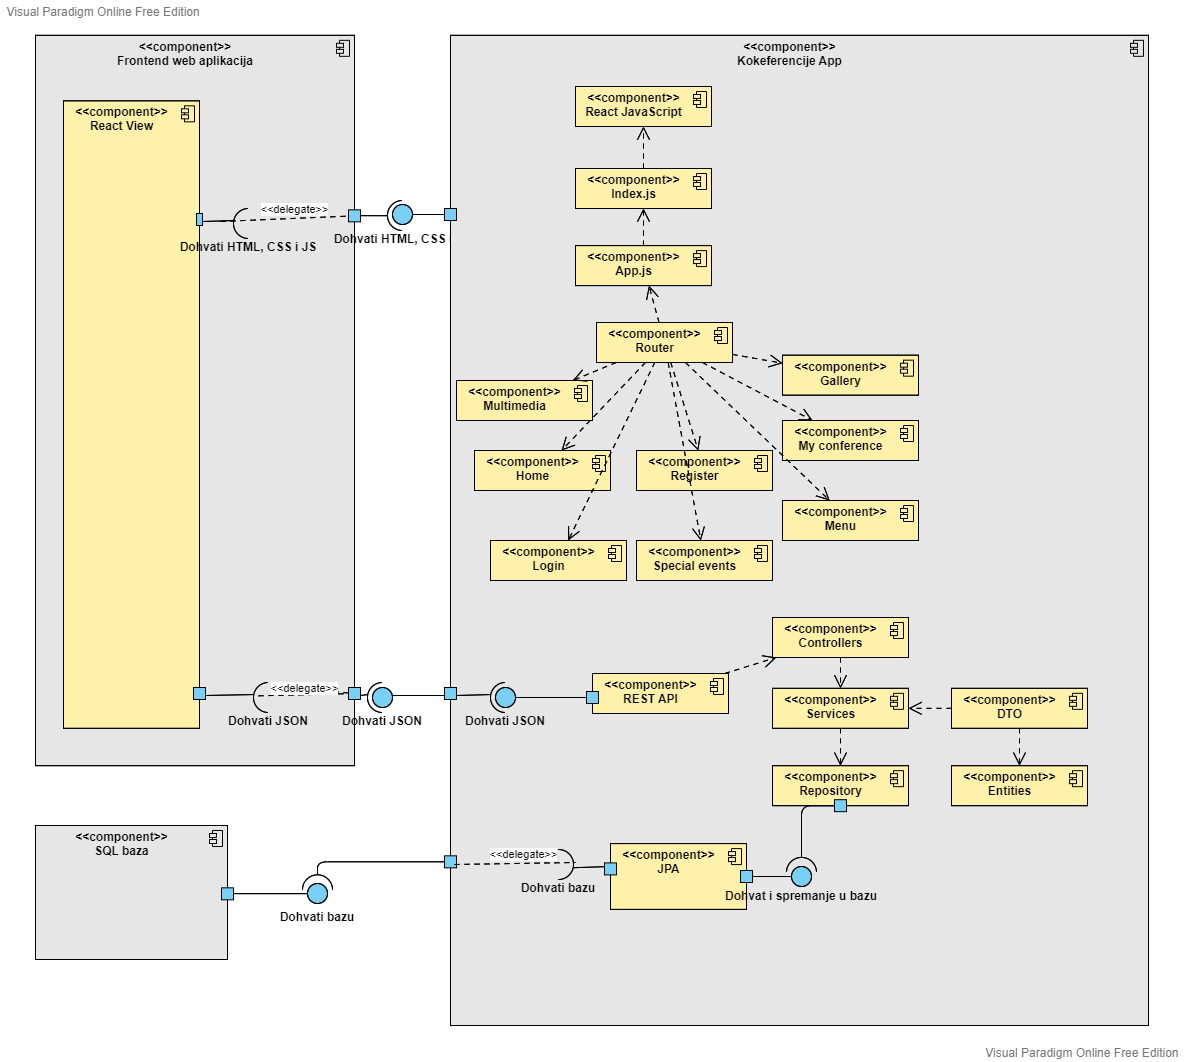
\includegraphics[scale=0.40]{slike/Dijagram_komp.png} %veličina slike u odnosu na originalnu datoteku i pozicija slike
			            \centering
			            \caption{Dijagram komponenti}
			            \label{fig:seq-dijagram2}
		        \end{figure}\\
				\eject